
%%%%%%%%%%%%%%%%%%%%%%% file typeinst.tex %%%%%%%%%%%%%%%%%%%%%%%%%
%
% This is the LaTeX source for the instructions to authors using
% the LaTeX document class 'llncs.cls' for contributions to
% the Lecture Notes in Computer Sciences series.
% http://www.springer.com/lncs       Springer Heidelberg 2006/05/04
%
% It may be used as a template for your own input - copy it
% to a new file with a new name and use it as the basis
% for your article.
%
% NB: the document class 'llncs' has its own and detailed documentation, see
% ftp://ftp.springer.de/data/pubftp/pub/tex/latex/llncs/latex2e/llncsdoc.pdf
%
%%%%%%%%%%%%%%%%%%%%%%%%%%%%%%%%%%%%%%%%%%%%%%%%%%%%%%%%%%%%%%%%%%%


\documentclass[runningheads,a4paper]{llncs2e/llncs}

\usepackage{amssymb,amsmath,bbm}
\setcounter{tocdepth}{3}
\usepackage{graphicx}

\usepackage{url}
\urldef{\mailjr}\path|juste.raimbault@polytechnique.edu|
\urldef{\mailjk}\path|julien.keutchayan@polytechnique.edu|
  
\newcommand{\keywords}[1]{\par\addvspace\baselineskip
\noindent\keywordname\enspace\ignorespaces#1}

\newcommand{\noun}[1]{\textsc{#1}}



\begin{document}

\mainmatter  % start of an individual contribution




% first the title is needed
\title{A Knowledge Framework}

% a short form should be given in case it is too long for the running head
\titlerunning{A Knowledge Framework}

% the name(s) of the author(s) follow(s) next
%
% NB: Chinese authors should write their first names(s) in front of
% their surnames. This ensures that the names appear correctly in
% the running heads and the author index.
%
\author{\noun{Juste Raimbault}$^{1,2}$}
%
\authorrunning{A Knowledge Framework}
% (feature abused for this document to repeat the title also on left hand pages)

% the affiliations are given next; don't give your e-mail address
% unless you accept that it will be published
\institute{$^{1}$ UMR CNRS 8504 G{\'e}ographie-Cit{\'e}s, Paris, France\\
$^{2}$ UMR-T IFSTTAR 9403 LVMT, Champs-sur-Marne, France\\
\mailjr
}

\toctitle{Lecture Notes in Computer Science}
\tocauthor{Authors' Instructions}
\maketitle


\begin{abstract}

\keywords{kw1, kw2}
\end{abstract}



%%%%%%%%%%%%%%%%
\section{Introduction}
%%%%%%%%%%%%%%%%

Relevant for complex systems, because fully reflexive : way of seeing the systems and the production of knowledge is itself rooted in complexity

https://arxiv.org/pdf/1704.01407.pdf : framework in AI (not knowledge framework)

\textbf{Cadres existants (exemples dans d'autres disciplines) : } \cite{carlile2004transferring} : sociologie de l'innovation ; \cite{durantin2017disruptive} : entre ingénierie et design ; \cite{gemino2004framework} : évaluation des grammaires dans les systèmes d'information ; \cite{cottineau2015modular} : Cadre de multi-modélisation pour le test d'hypothèses.


\cite{raimbault:halshs-01505084}






%%%%%%%%%%%%%%%%
\section{Case Studies}
%%%%%%%%%%%%%%%%


%%%%%%%%%%%%%%%%
\subsection{Genesis of the Evolutive Urban Theory}
% -  incl. figure nw ?

The first case study relates the construction of the \emph{Evolutive Urban Theory}, a geographical theory to study territorial systems

\cite{legavre1996neutralite} % methodology semi-directive interview



%%%%%%%%%%%%%%%%
\subsection{Engineering the Metropolitan}

After the glance on domains of knowledge extracted in the previous case study, we propose to take the corresponding point of view on a rather different example more related to technology and engineering


\cite{belmonte2008automatisation} automatisation de la 1 \cite{foot2005faut} portes palières
% http://cat.inist.fr/?aModele=afficheN&cpsidt=17871610
% http://cat.inist.fr/?aModele=afficheN&cpsidt=3212393 : meteor

\cite{hatchuel1988stations} innovation stations

\cite{foot1994ratp} conflits sociaux ratp

\cite{moreno2016etude} ingénierie des tunnels

\cite{balbo2016positionnement} multi-agent systems and autonomous intelligent transportation systems



%%%%%%%%%%%%%%%%
\section{Knowledge Framework}
%%%%%%%%%%%%%%%%


From the previous analyses, we can formulate know inductively the knowledge framework. As mentioned, it takes the idea of interacting domains of knowledge from the framework introduced by~\cite{livet2010}, but extends these domains and takes a novel epistemological position, focusing on co-evolutive dynamics of agents and knowledge.


\paragraph{Constraints}

To be particularly fitted for the study and management of complexity

%  - constraints
% Intégration des disciplines (objets géographiques par nature interdisciplinaires)
% Intégration des domaines de connaissance : pas de composante privilégiée
% Au delà des frontières artificielles ``quantitatif-qualitatif'' : intégration des méthodes

% - initial framework : \cite{livet2010}

% - Epistemological fundations
% Une approche cognitive de la Science~\cite{giere2010explaining} : les \textit{agents} scientifiques~\cite{giere2010agent} à l'origine des dynamiques co-évolutives des connaissances. Cadre épistémologique du perspectivisme~\cite{giere2010scientific}.
% Compatible avec une \textit{science anarchiste} à la Feyerabend \cite{feyerabend1993against} : auto-organisation et émergence des connaissances
% 3. Extrême sur la ``check-list'' de Hacking~\cite{hacking1999social} (au delà de Kuhn) :
% - contingence maximale de par la nature dépendante au chemin du processus complexe de co-évolution des connaissances
% - degré de constructivisme maximal dans la posture perspectiviste
% - stabilité des sciences fortement couplée entre origine interne et externe de par le rôle des agents

\paragraph{Epistemological Fundations}

Our epistemological positioning relies on a cognitive approach to science, given by Giere in~\cite{giere2010explaining}

% - formulation
%\textbf{Definition.} La morphogenèse d'un système implique des relations circulaires causales et souvent autonomes entre les niveaux d'émergence\\ (\cite{bedau2002downward}) entre \textit{forme} et \textit{fonction} \cite{antelope2016interdisciplinary}, et exhibe dans ce sens une architecture émergente \cite{doursat2012morphogenetic}.

%\textbf{Fait stylisé.} Il existe des processus de production de connaissances scientifiques morphogénétiques, constitués d'ensemble de \textit{perspectives}, et impliquant une co-évolution des vecteurs (agents) et de domaines de connaissance (def. ci-dessous).

% \item \textbf{Empirique} Connaissances empiriques sur des cas réels
% \item \textbf{Théorique} Construction cognitives plus générales
% \item \textbf{Modélisation} \textit{Medium} formalisé de la perspective, ou tout modèle au sens de Varenne \cite{varenne2010simulations}
% \item \textbf{Données} Information brute qui a été captée
% \item \textbf{Méthodes} Structures génériques de production de connaissances
% \item \textbf{Outils} Proto-méthodes et supports des autres domaines

% \textbf{Corolaire.} La distinction entre ``quantitatif'' et ``qualitatif'' est arbitraire et sans intérêt pour la production dans ce cadre, de par la nécessité de l'ensemble de leur composantes dans l'ensemble des domaines.  

% Modèles
% Modèles de simulation
% Modèles statistiques ou mathématiques
% Modèles de données
% Modèles conceptuels



%%%%%%%%%%%%%%%%
\begin{figure}
\centering
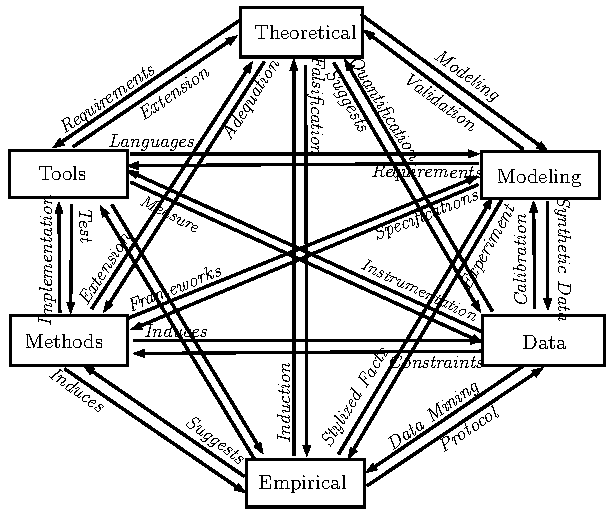
\includegraphics[width=\textwidth]{figures/framework}
\caption{\textbf{Projection of a perspective into a full network of knowledge domains}}
\label{fig:fwk}
\end{figure}
%%%%%%%%%%%%%%%%




%%%%%%%%%%%%%%%%
\section{Discussion}
%%%%%%%%%%%%%%%%



%%%%%%%%%%%%%%%%
\subsection{Application Range}

We insist that our framework does not pretend to introduce a general epistemology of scientific knowledge as Kant has tried to construct with the Critique of Pure Reason, but far from that is rather targeted towards reflexivity in the understanding of complex systems. The level of generality is at a very different level, but the aim to practical implication in the handling of complexity contributes to a certain genericity in applications. It is furthermore particularly suited to study Complex Systems, since more reductionist approaches can handle more compartmented production of knowledge, whereas integration of disciplines and scales and therefore domains of knowledge has been emphasized as crucial 


%%%%%%%%%%%%%%%%
\subsection{Towards a formalisation}

Our knowledge framework stays at an epistemological level, and its application must 









%%%%%%%%%%%%%%%%
\section{Conclusion}
%%%%%%%%%%%%%%%%




\section*{Acknowledgments}

The author would like to thank D. Pumain and R. Reuillon for giving of their time for the interviews.



%%%%%%%%%%%%%%%%
%% Biblio
%%%%%%%%%%%%%%%%

\bibliographystyle{unsrt}
\bibliography{biblio/biblio,/Users/Juste/Documents/ComplexSystems/CityNetwork/Biblio/BibTeX/CityNetwork}





\end{document}
